\documentclass[10pt,french]{article}
\input preambule_2013

\newcounter{exoc}
\newenvironment{exoc}[1]{%
  \refstepcounter{exoc}\textbf{Exercice \theexoc} :\hfill {\footnotesize\textbf{(#1)}}\par
  \medskip}%
{\medskip}

\pagestyle{fancy}
\pieddepage{}{\thepage}{}

\setlength{\textheight}{26cm}% Hauteur de la zone de texte

\newcommand\resultat[1]{\pfr{#1}}

\begin{document}

\begin{center}
\begin{tabularx}{\textwidth}{|>\centering m{2.5cm}|>\centering X|>{\centering\arraybackslash} m{2.5cm}|}
	\hline
		1\iere \bsc{s.t.m.g.} &  Mercredi 30 avril \np{2014} & \textbf{Bilan annuel} \\
	\hline
		\multicolumn{3}{|c|}{\bsc{Correction}} \\
	\hline
\end{tabularx}
\end{center}\bigskip

\begin{exoc}{3 points}
Les justifications n'étaient pas exigées.
    \begin{enumerate}
        \item Le taux $t$ est égal à $180\%$. D'après le cours, on multiplie la valeur par $1 + t$ donc par $1+1,80$ donc :\par
            \textbf{Réponse c :} Il a été multiplié par $2,80$.
        \item $t = 25\%$. Le taux réciproque $t'$ est tel que : $1 + t' = \dfrac{1}{1 + t}$. Ici, $\dfrac{1}{1+t} = \dfrac{1}{1 + 0,25} = 0,8$.\par Ainsi, $1 + t' = 0,8$ donc $t' = 0,8 - 1$ donc :\par
            \textbf{Réponse a :} $-20\%$.
        \item Le taux d'évolution global $t$ est tel que $1 + t = (1 + t_1)(1 + t_2)$ avec ici $t_1 = +5\%$ et $t_2 = -2\%$.\par
        Ainsi : $1 + t = (1+0,05)(1-0,02) = 1,029$ donc $t = 1,029 - 1 = 0,029$. Donc :\par
            \textbf{Réponse d :} $+ 2,90\%$.
    \end{enumerate}
\end{exoc}
\[*\]

\begin{exoc}{6 points}
    \begin{enumerate}
        \item $u_1$ est le nombre d'adolescents ayant regardé l'émission la première semaine. D'après l'énoncé, \resultat{$u_1 = 400$}.
        
        \item La semaine suivante, l'audience a augmenté de $5\%$ donc $u_2 = u_1(1 + 5\%) = 400 \times 1,05 = 420$.\par
        \resultat{$u_2 = 420$}. La deuxième semaine, $420$ adolescents ont regardé l'émission.\par
        De même $u_3 = u_2(1 + 5\%) = 420 \times 1,05 = 441$.\par \resultat{$u_3 = 441$}. La troisième semaine, $441$ adolescents ont regardé l'émission.
        
        \item En suivant la logique précédente, \resultat{$u_{n+1} = u_n \times 1,05$}.
        
        \item D'après le cours, la suite \resultat{$(u_n)$ est une suite géométrique} de raison $q = 1,05$ et de premier terme $u_1 = 400$. En effet, pour passer d'un terme au terme suivant, on multiplie toujours par le même nombre $1,05$.
        
        \item On sait que $u_2 = u_1 \times 1,05$. De même $u_3 = u_2 \times 1,05 = \underbrace{u_1 \times 1,05}_{\tiny u_2} \times 1,05 = u_1 \times 1,05^2$.\par
        Par le même raisonnement, on a : $u_4 = u_3 \times 1,05 = \underbrace{u_1 \times 1,05^2}_{\tiny u_3} \times 1,05 = u_1 \times 1,05^3$.\par
        On continue jusqu'à obtenir \resultat{$u_n = u_1 \times 1,05^{n-1}$}.
        
        \item Le nombre d'adolescents regardant l'émission lors de la douzième semaine est égal à $u_{12}$.\par
        D'après la formule précédente, $u_{12} = u_1 \times 1,05^{11} \approx 684$. Le tableau de valeur de la calculatrice permet d'obtenir le même résultat.\par
        \resultat{$u_{12} \approx 684$}. La finale a été regardé par $684$ adolescents la douzième semaine.
    \end{enumerate}
\end{exoc}
\[*\]

\begin{exoc}{7 points}
    %----------------------------------------------------------------------------
    \textbf{Partie} \rond{A}\quad Lectures graphiques\medskip
    %-----------------------------------------------------------------------------

    \begin{enumerate}
        \item Le coût de fabrication de $6$ meubles revient à \resultat{\EUR{$600$}}.\par
                 Le coût de fabrication de $13$ meubles revient à \resultat{\EUR{$\np{2000}$}}.

        \item Pour $x = 13$, la courbe $\calig C$ est au-dessus de la courbe $\calig R$ donc le coût de fabrication de $13$ meubles est supérieur à la recette obtenue en vendant les meubles. Donc \resultat{ce n'est pas rentable} pour l'artisan de fabriquer et vendre $13$ meubles.

        \item Pour un coût de fabrication de \EUR{$900$}, l'artisan peut fabriquer \resultat{$8$ meubles}.

        \item Le bénéfice est positif lorsque la courbe $\calig R$ est au-dessus de la courbe $\calig C$. Cela est vrai sur l'intervalle $\intervalleff{1,5}{12,5}$ (valeurs approchées). Le nombre de meubles à construire est évidemment un nombre entier.\par
            Pour être bénéficiaire, l'entreprise doit donc construire \resultat{entre $2$ et $12$ meubles}.
    \end{enumerate}

    \begin{center}
    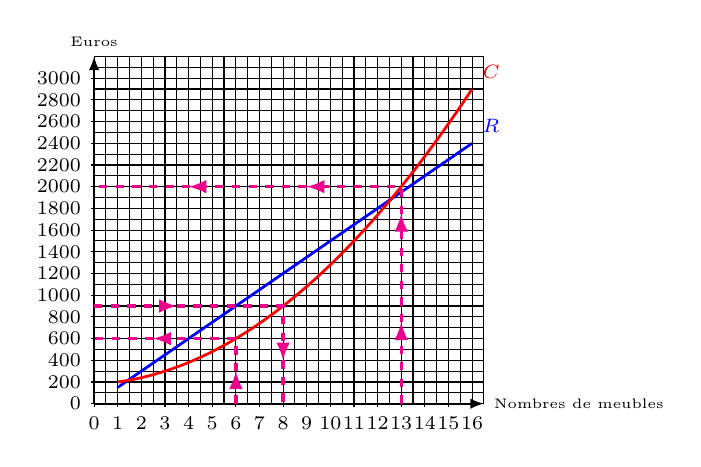
\begin{tikzpicture}[>=latex,x=1cm,y=0.0046cm,scale=0.3]
        \draw[line width = 0.4pt] (0,0) grid[xstep=0.5,ystep=100] (16.5,3200);
        \draw[->,line width=0.7pt] (0,0) -- (16.5,0) node[right] {\tiny Nombres de meubles};
        \draw[->,line width = 0.7pt] (0,0) -- (0,3200) node[above] {\tiny Euros};
        \draw[line width=1pt,blue] plot[domain=1:16,samples=200] (\x,{150*(\x)}) node[above right]{\scriptsize $\calig R$};
        \draw[line width=1pt,red] plot[domain=1:16,samples=200] (\x,{10*(\x)^2+10*\x+180}) node[above right]{\scriptsize $\calig C$};
        \foreach \x in {0,...,16} \draw (\x,0)--(\x,-4pt) node[below] {\scriptsize $\x$};
        \foreach \x in {0,200,...,3000} \draw (0,\x)--(-4pt,\x) node[left] {\scriptsize $\x$};
        \draw[magenta,dashed,line width = 1.2pt,->] (6,0) -- (6,300);
            \draw[magenta,dashed,line width = 1.2pt,->] (6,300) -- (6,600) -- (2.5,600);
            \draw[magenta,dashed,line width = 1.2pt] (2.5,600) -- (0,600);
        \draw[magenta,dashed,line width = 1.2pt,->] (13,0) -- (13,750);
            \draw[magenta,dashed,line width = 1.2pt,->] (13,750) -- (13,1750);
            \draw[magenta,dashed,line width = 1.2pt,->] (13,1750) -- (13,2000) -- (9,2000);
            \draw[magenta,dashed,line width = 1.2pt,->] (9,2000) -- (4,2000);
            \draw[magenta,dashed,line width = 1.2pt] (9,2000) -- (0,2000);
        \draw[magenta,dashed,line width = 1.2pt,->] (0,900) -- (3.5,900);
            \draw[magenta,dashed,line width = 1.2pt,->] (3.5,900) -- (8,900) -- (8,400);
            \draw[magenta,dashed,line width = 1.2pt] (8,400) -- (8,0);
    \end{tikzpicture}
    \end{center}

    %----------------------------------------------------------------------------
    \textbf{Partie} \rond{B}\quad \'Etude du bénéfice\medskip
    %----------------------------------------------------------------------------

    \begin{enumerate}
        \item $B(x) = -10x^2 + 140x - 180$ avec $a = -10$. Sur $\R$, on a donc le tableau de variations suivant :
            \begin{center}
                \begin{tikzpicture}[scale=0.7]
                    \tkzTabInit[nocadre,espcl=2.5]{$x$/0.75,\small Variations \\ de $B$/1.5}{$-\infty$,,$+\infty$}
                    \tkzTabVar{-/,+/,-/}
                \end{tikzpicture}
            \end{center}

        \item Le maximum est obtenu pour $x = \dfrac{-b}{2a} = \dfrac{-140}{2 \times (-10)} = 7$.\par
        Pour que le bénéfice soit maximal, il faut fabriquer \resultat{$7$ meubles}.

        \item $B(7) = -10\times 7^2 + 140 \times 7 - 180 = -490 + 980 - 180 = 310$.\par
        Le bénéfice maximal est égal à \resultat{\EUR{$310$}}.

        \item $\Delta = b^2 - 4ac$ avec $a = -10$, $b=140$ et $c = -180$ donc $\Delta = 140^2 - 4 \times (-10) \times (-180) = \np{12400}$.\par
        Le discriminant de $B$ est positif donc l'équation $B(x) = 0$ admet deux solutions :
        \[\begin{array}[t]{rcl}
            x_1 & = & \dfrac{-b - \sqrt \Delta}{2a} \\[8pt]
                   & = & \dfrac{-140 - \sqrt{\np{12400}}}{2 \times (-10)} \\[8pt]
                   & \approx & 12,6
        \end{array}
        \qetq
        \begin{array}[t]{rcl}
            x_2 & = & \dfrac{-b + \sqrt \Delta}{2a} \\[8pt]
                   & = & \dfrac{-140 + \sqrt{\np{12400}}}{2 \times (-10)} \\[8pt]
                   & \approx & 1,4
        \end{array}\]
       Les solutions de l'équation $B(x) = 0$ sont donc (au dixième près) : \resultat{$1,4$ et $12,6$}.
    \end{enumerate}
\end{exoc}
\[*\]

\begin{exoc}{4 points}
    \begin{minipage}{0.52\linewidth}
        \begin{enumerate}
            \item Il y a $80$ biscuits dont $40$ à la vanille et $24$ à l'orange. Le reste est à la noix de coco. Puisque $80 - 40 - 24 = 16$, il y a $16$ biscuits à la noix de coco.\par
            Donc : \resultat{$p(N) = \dfrac{16}{80} = 0,2$}.

            \item voir ci-contre
            
            \item $V \cap C$ est l'événement : << obtenir un biscuit à la vanille avec des pépites de chocolat >>. On suit le chemin de l'arbre $V \rightarrow C$ donc :
            $p(V \cap C) = \dfrac{40}{80} \times \dfrac{60}{100} = \dfrac{\np{2400}}{\np{8000}}.$
            Ainsi, \resultat{$p(V \cap C) = 0,3$}.
            
            \item Il y a trois chemins pour obtenir un biscuit avec des pépites de chocolat : $V \cap C$, $O \cap C$ et $N \cap C$. Ainsi,
            \[\begin{array}{r@{\ =\ }c@{\ +\ }c@{\ +\ }c}
                p(C) & p(V \cap C) & p(O \cap C) & p(N \cap C) \\
                        & \dfrac{40}{80} \times \dfrac{60}{100} & \dfrac{24}{80} \times \dfrac{25}{100} & \dfrac{16}{80} \times 0\\
                        & 0,3 & 0,075 & 0 \\
                \multicolumn{4}{l}{\resultat{p(C) = 0,375}}
                \end{array}\]
        \end{enumerate}
    \end{minipage}\hfill
    \begin{minipage}{0.45\linewidth}
            \tikzstyle{level 1}=[level distance=2cm,sibling distance=-3cm]
            \tikzstyle{level 2}=[level distance=2.5cm,sibling distance=-1.5cm]
         \begin{center}
            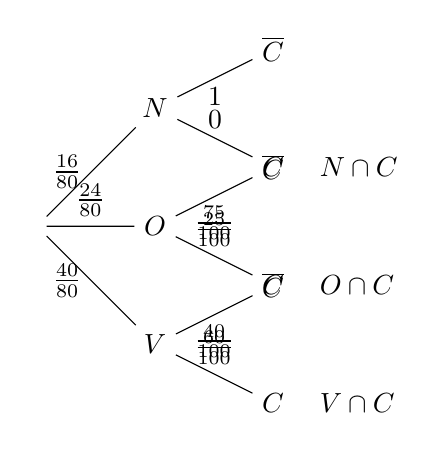
\begin{tikzpicture}
            [grow=right] % dessine l'arbre de gauche à droite. Les options left, up et down sont également disponibles.
                \node{}
            %----------------------------------------------------------------------------------------------------------------------
            %----------------------------------------------------------------------------------------------------------------------
                    child {node {$V$}
            %----------------------------------------------------------------------------------------------------------------------
                            child {node {$C$}
                                      node[right = 1em] {$\rightsquigarrow\ V\cap C$}
                                     edge from parent node[above] {$\frac{60}{100}$}
                                    }
            %----------------------------------------------------------------------------------------------------------------------
                            child {node {$\overline C$}
                                     edge from parent node[below] {$\frac{40}{100}$}
                                    }
            %----------------------------------------------------------------------------------------------------------------------
                       edge from parent node[left] {$\frac{40}{80}$}
                    }
            %----------------------------------------------------------------------------------------------------------------------
            %----------------------------------------------------------------------------------------------------------------------
                    child {node {$O$}
            %----------------------------------------------------------------------------------------------------------------------
                            child {node {$C$}
                                      node[right = 1em] {$\rightsquigarrow\ O\cap C$}
                                     edge from parent node[above] {$\frac{25}{100}$}
                                    }
            %----------------------------------------------------------------------------------------------------------------------
                            child {node {$\overline C$}
                                     edge from parent node[below] {$\frac{75}{100}$}
                                    }
            %----------------------------------------------------------------------------------------------------------------------
                        edge from parent node[above] {$\frac{24}{80}$}
                    }
            %----------------------------------------------------------------------------------------------------------------------
            %----------------------------------------------------------------------------------------------------------------------
                    child {node {$N$}
            %----------------------------------------------------------------------------------------------------------------------
                            child {node {$C$}
                                      node[right = 1em] {$\rightsquigarrow\ N\cap C$}
                                     edge from parent node[above] {$0$}
                                    }
            %----------------------------------------------------------------------------------------------------------------------
                            child {node {$\overline C$}
                                     edge from parent node[below] {$1$}
                                    }
            %----------------------------------------------------------------------------------------------------------------------
                        edge from parent node[left] {$\frac{16}{80}$}
                    }
            ;
            \end{tikzpicture}
        \end{center}
    \end{minipage}
\end{exoc}


\end{document} 